\chapter{Concept for an Exergame for Elderly}


\begin{figure} [ht!]
\centering
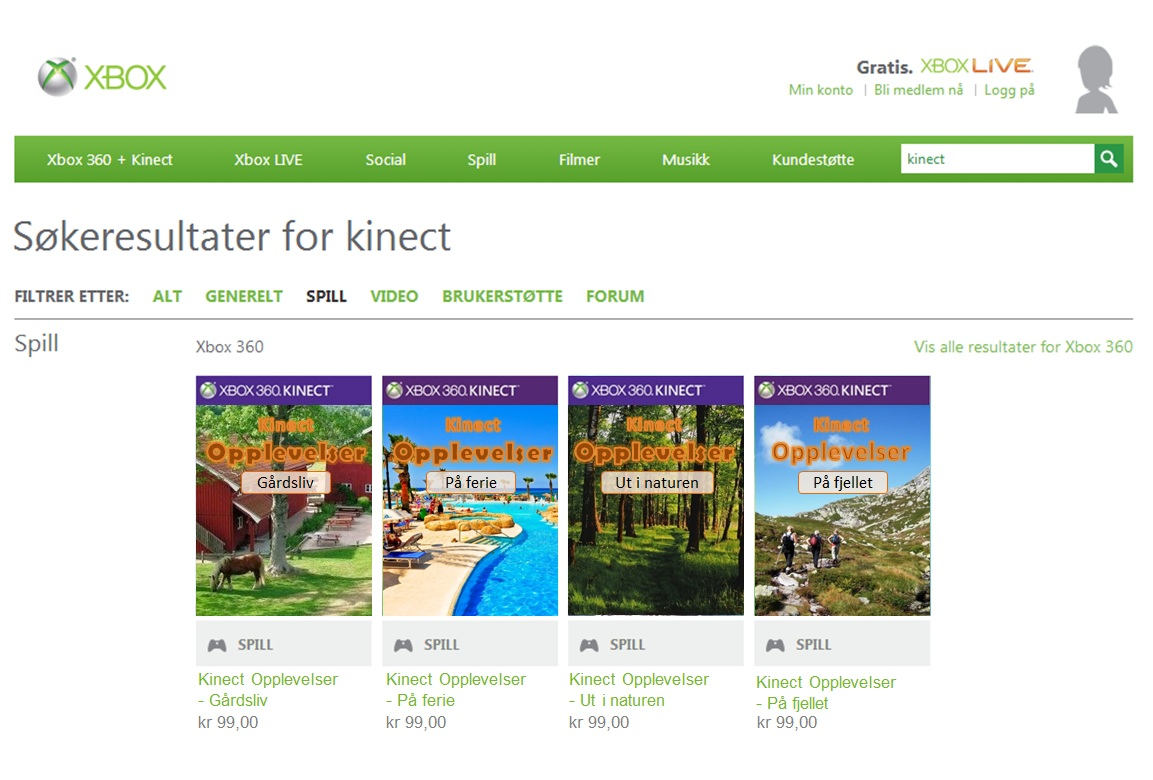
\includegraphics[scale=0.5, angle=90]{SpillXboxNYNY.jpg}
\caption[Presentation of our video game series]{A presentation of how our video game series would look like on Xbox's website [modified from \cite{XboxNettside}].}
\label{videogameseries}
\end{figure}

\begin{figure} [ht!]
\centering
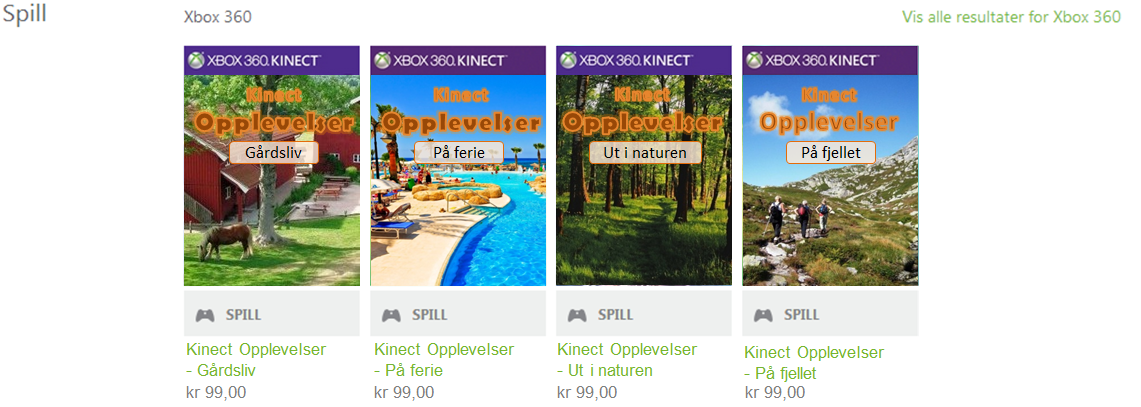
\includegraphics[scale=0.7, angle=90]{SpillXboxNY.png}
\caption[Presentation of our video game series]{A presentation of how our video game series would look like on Xbox's website [modified from \cite{XboxNettside}].}
\label{videogameseries}
\end{figure}

\begin{figure} [ht!]
\centering
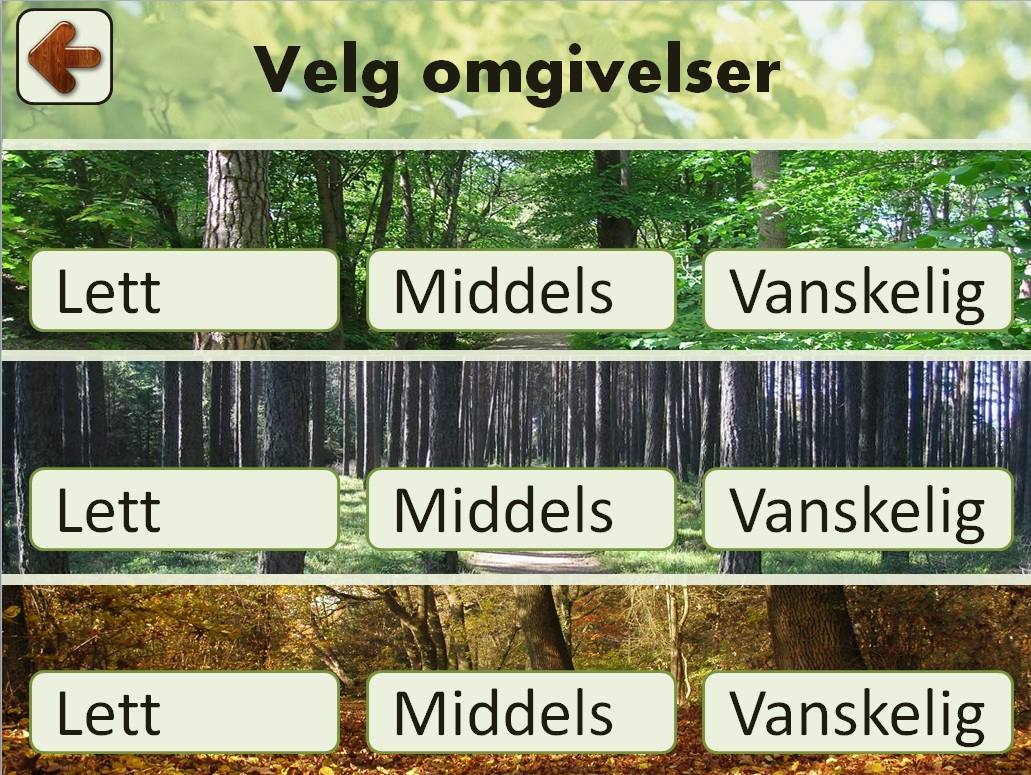
\includegraphics[scale=0.45]{VelgOmgivelser.jpg}
\caption[Choice of surroundings and difficulty]{When "Take a walk in the nature" is chosen, players will get the possibility to choose surroundings and difficulty level.}
\label{omgivelseNivaa}
\end{figure}

\begin{figure} [ht!]
\centering
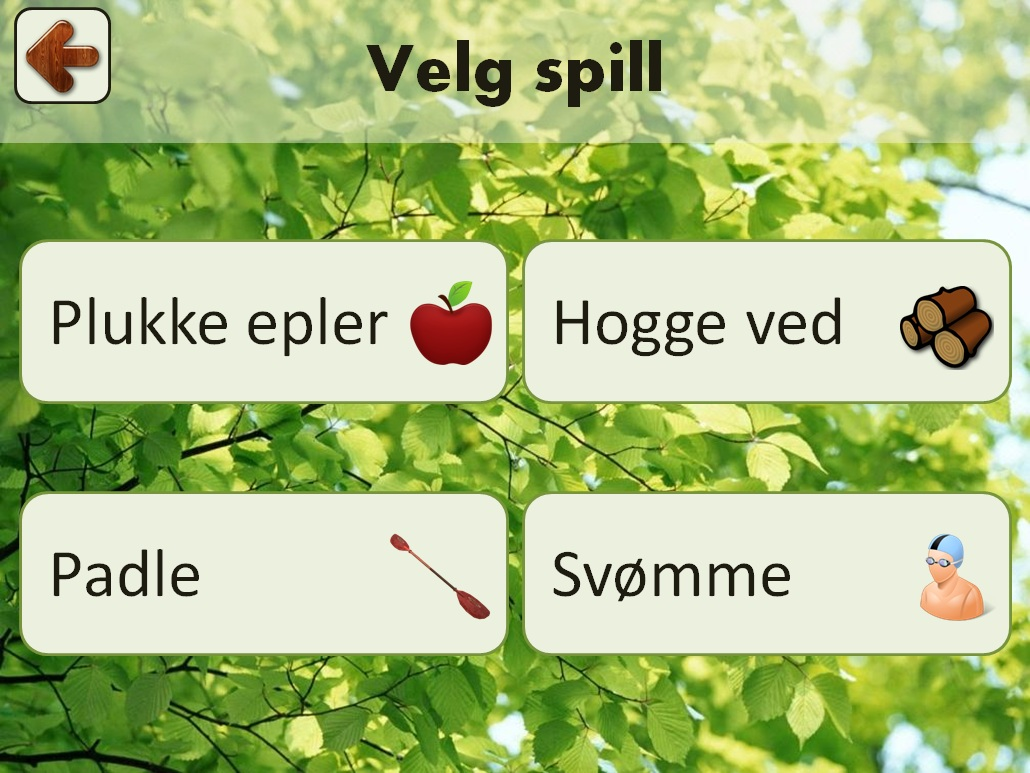
\includegraphics[scale=0.4]{VelgSpill.jpg}
\caption[The four single games]{Besides the walk in the nature the players can choose between four single games, picking apples, chopping wood, paddling, and swimming.}
\label{velgSpill}
\end{figure}

\begin{figure} [ht!]
\centering
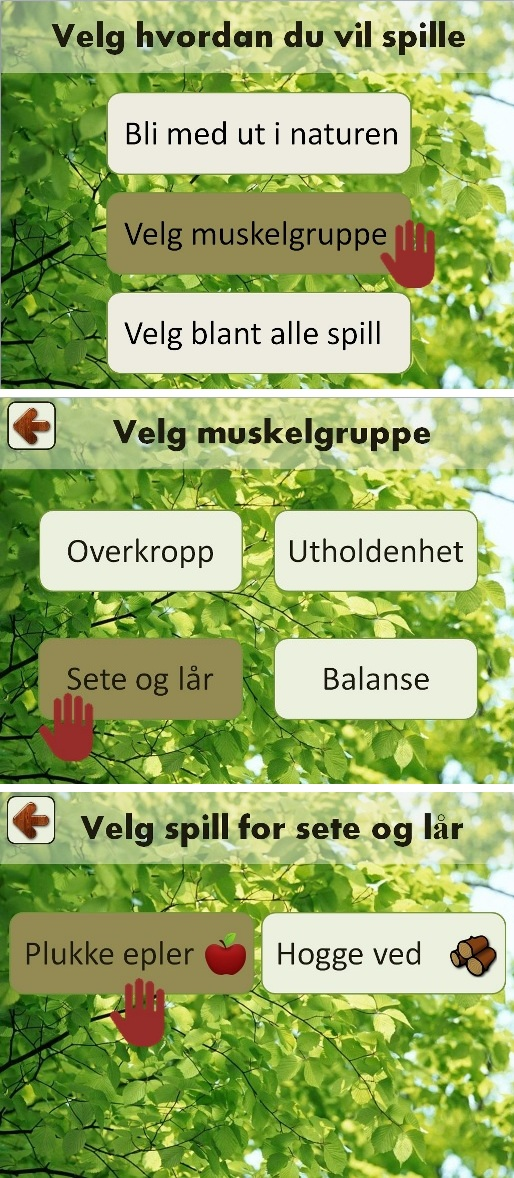
\includegraphics[scale=0.5]{menuStep1.jpg}
\caption[The menu, part one]{This figure shows the menu step by step, from the beginning to playing a single game, here picking apples. The selection of single games is a result of the chosen muscle group.}
\label{menu1}
\end{figure}

\begin{figure} [ht!]
\centering
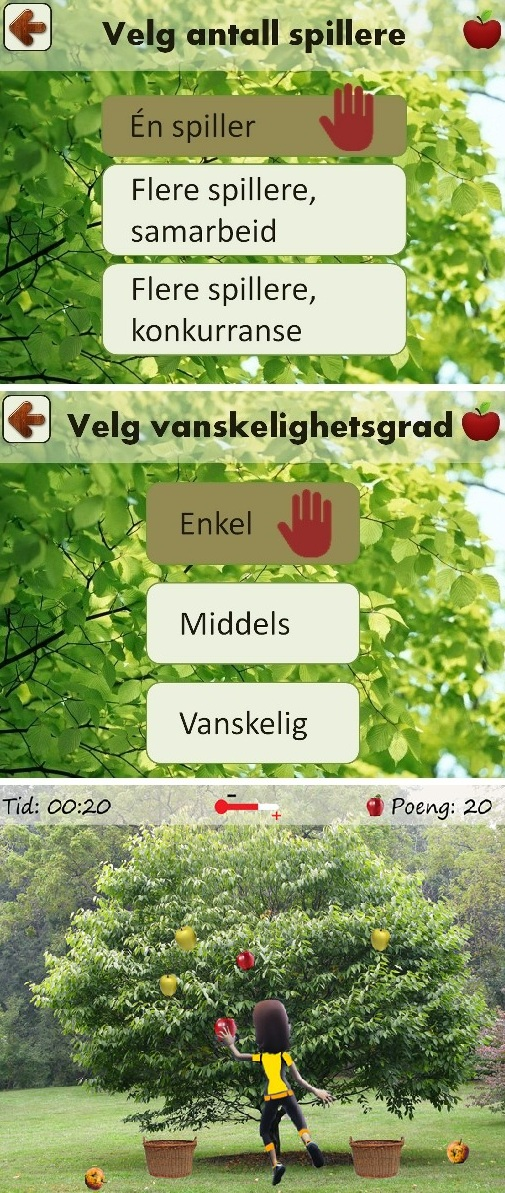
\includegraphics[scale=0.5]{menuStep2.jpg}
\caption[The menu, part two]{This figure shows the menu step by step, from the beginning to playing a single game, here picking apples. Single player game and difficulty level easy are chosen.}
\label{menu2}
\end{figure}